%%----------Chapter 2------------------------------------------
\chapter{Literature Review}
we started literature review from top research-general like IEEE, ACM and Nero-computing. i have try to review mostly citation papers with impact factor also prefer author contribution in my research topic. i tried to read maximum research paper not only high impact.  


\section{SAMPLING THE OUTPUT}
\label{sec:sample}

In the remainder of the paper we will refer to the RNN algorithm implemented in \cite{hidasi2015session} as GRU4Rec, the name of the implementation published by the authors on github \footnote{https://github.com/hidasib/GRU4Rec}
. In this

section we revisit how GRU4Rec samples negative feedback on the output and discuss its importance. We extend this sampling with an option for additional samples and argue that this is crucial
for the increased recommendation accuracy we achieve (up to 51\% improvement).


In each training step, GRU4Rec takes the item of the current event in the session – represented
by a one-hot vector – as an input. The output of the network is a set of scores over the items,
corresponding to their likelihood of being the next item in the session. The training iterates through
all events in the sequence. The complexity of the training with backpropagation through time is
O(NE(H2 + HNO)) where NE is the number of training events, H is the number of hidden units
and NO is the number of outputs, for which scores are computed. Computing scores for all items
is very impractical, since it makes the network unscalable \footnote[2]{While it can still result in an acceptable training time for smaller datasets, especially if the number of items
is only a few tens of thousand, algorithms scaling with the product of the number of events and items cannot
scale up for larger datasets}
. Therefore GRU4Rec uses a sampling
mechanism and during training computes the scores for a subset of the items only.

Instead of making a forward and backward pass with one training example only and then moving
to the next, the network is fed with a bundle of examples and is trained on the mean gradient. This
common practice is called mini-batch training and has several benefits, e.g. utilizing the parallelization capabilities of current hardware better, thus training faster, and producing more stable gradients
than stochastic gradient training and thus converging faster. GRU4Rec introduced mini-batch based
sampling \cite{hidasi2015session}. For each example in the mini-batch, the other examples of the same
mini-batch serve as negative examples (see Figure \ref{fig:p1}).\footnote[3]{
e.g.: Assume a mini-batch of 32 examples, with one desired output (target) for each example. Scores are
computed for all 32 items for each of the 32 examples resulting in 32 × 32 = 1024 scores. Thus we have 31
scores of negative examples for each of the targets.} 
This method is practical from an implementation point of view and can be also implemented efficiently for GPUs.

\graphicspath{{img/}}

\begin{figure}[htp]
    \centering
    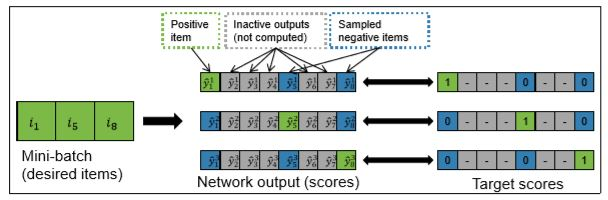
\includegraphics[width=400]{img/p1.JPG}
    \caption{Median negative gradients of BPR and BPR-max w.r.t. the target score against the rank of the target item. Left: only mini batch samples are used (mini batch size: 32); Center: 2048 additional negative samples were added to the mini batch samples; Right: same setting as the center, focusing on ranks 0-200.}
    \label{fig:p1}
\end{figure}

The network can be trained with one of three different listwise ranking loss functions (see Section 3).
All loss functions require a score for the target item (i.e. for the item which was the actual next
item) and score(s) for at least one negative sample (i.e. item other than the target). One property
of ranking losses is that learning happens only if the score of the target item does not exceed that
of the negative samples by a large margin, otherwise the items are already in the right order, so
there is nothing to be learned. Therefore, when utilizing a sampling procedure, it is crucial that
high scoring items make it among the negative samples. Whether an item has a high score, depends
on the context (item sequence) the scores are actually computed for. Popular items generally score
high in many situations, making popularity-based sampling a good sampling strategy. Mini-batch
sampling is basically a form of popularity-based sampling, since the training iterates through all
events, thus the probability of an item acting as a negative sample is proportional to its support. The
problem with popularity-based sampling is that learning can slow down after the algorithm learns
to (generally) rank target items above popular ones, and thus can still be inaccurate with ranking
long tail high scoring items. On the other hand, uniform sampling slows down learning, due to the
high number of low scoring negative samples, but might produce an overall more accurate model if
trained indefinitely. In our experience, popularity-based sampling generally produces better results.

Tying sampling to the mini-batches has several practical benefits, but is too restrictive for three
reasons. (1) Mini-batch sizes are generally small, ranging from few tens to few hundreds. If the
number of items is large, the small sample size further hinders the chance of including all of the high
scoring negative examples. (2) Mini-batch size has a direct effect on the training. E.g. we found that training with smaller mini-batch sizes (30-100) produces more accurate models, but training
with larger ones is faster on the GPU due to parallelization. (3) The sampling method is inherently
popularity-based, which generally is a good strategy, but might not be optimal for all datasets.

Therefore we extend the sampling of GRU4Rec with additional samples. We sample NA items
which are shared by the examples of the mini-batch, i.e. the same samples are used for each example \footnote[4]{However, the scores of these samples will be still different per example, because of the differing item sequences they are based on.}. These additional samples are used along with the NB $ − 1$ samples coming from the mini-batch (popularity) sampling. Additional samples can be sampled in any way, we chose to sample proportional to $supp^\alpha_i$, where $supp^{\alpha}_{i}$ is the support of the item and $\alpha$ is the parameter of the sampling. $\alpha = 0$ and $\alpha = 1$ gives uniform and popularity-based sampling respectively.

Adding more samples naturally increases the complexity, since NO increases from NB to NA + NB.However, the computations are easily parallelizable, thus there is no actual increase in the training
time on modern GPUs up to a certain sample size (see Section 4.1). The efficient implementation of this sampling however is not trivial. Sampling according to a distribution on GPUs is slow, thus it should be handled by the CPU. The sampled item IDs can be given to the GPU along with the item IDs of the mini-batch. Sampling the distribution takes some time every time a new mini batch is formed, thus GPU execution is frequently interrupted, making GPU utilization low and thus training slow. On the top of that, sampling a few items at once is less efficient than sampling lots of them, even on CPU. Therefore we implemented a cache that pre-samples and stores lots of negative
samples. Training uses up these samples and the cache is recomputed once it is empty. We found that pre-sampling 10-100 million item IDs significantly improves training speed when compared to using no cache at all.



\section{Example List}
\subsection{Example Dotted List}
%%-----------------example dotted list--------------------
\smallskip
\textbf{Some special characters in TeX:}
\begin{itemize}
\item Accents
\item Braces
\item Dollar signs
\end{itemize}

\subsection{Example Numbered List}
%%----------------example numbered list---------------------
\smallskip
\textbf{Some special characters in TeX:}
\begin{enumerate}
\item Accents
\item Braces
\item Dollar signs
\end{enumerate}

\section{Math Example}
\subsection{Inline Math Mode}
%%-------------------example math equation----------
Mathematical material to be typeset inline must be surrounded by a
single dollar sign. For example: $a^2 + b^2 = c^2$.
\subsection{Displayed Math}
This is a displayed math example without numbering.
\[
\lim_{x \to a}f(x)
\]

\[
\left|\sum_{i=1}^n a_ib_i\right| \le \left(\sum_{i=1}^n
a_i^2\right)^{1/2} \left(\sum_{i=1}^n b_i^2\right)^{1/2}
\]

This is a math equation with numbering.
\begin{equation}
(a+b)^3 = (a+b)^2(a+b)
\end{equation}

%%-----------------example aligned equation------------------
This is multiline equation example.
\begin{align}
(a+b)^3 &= (a+b)^2(a+b)\\
&=(a^2+2ab+b^2)(a+b)\\
&=(a^3+2a^2b+ab^2) + (a^2b+2ab^2+b^3)\\
&=a^3+3a^2b+3ab^2+b^3
\end{align}

%%--------------example matrix-------------------------------
This is a matrix
\[
\begin{matrix}
    a+b & uv & x-y & 5\\
    a+b+c & u+v &x+y & 10
\end{matrix}
\]

%%------------example cases----------------------------------
This is a case
\[
f(x)=
\begin{cases}
    -x^{2}, &\text{if $x<0$;}\\
    \alpha+x, &\text{if $0 \leq x \leq 1$;}\\
    x^{2}, &\text{otherwise.}
\end{cases}
\]

%%--------------------example figure-------------------
\section{Graphics Example}
\subsection{Stars}
The ideal graphics format for inclusion in a \LaTeX document is
"encapsulated postscript" or eps. Here is an example figure.
\begin{figure}[htbp]
\begin{center}

\includegraphics[width=\textwidth]{Stars}
\caption{Stars}
\end{center}
\end{figure}